\subsubsection{Pooling Layer}
\label{sec:cnn-pooling-layer}
After obtaining features using a convolutional layer a pooling layer can be inserted working on their activations.
Pooling serves as a sample-based discretization process.
This is done by moving a filter $\vec{K} \in \mathbb{R}^{i \times j}$ with an arbitrary stride $s$ over an input $\vec{I} \in \mathbb{R}^{u \times v}$ that compresses the information or values, respectively, within its window.
The result is a reduction of the inputs spatial dimensions.
However, the depth is usually not compressed and stays the same.
The objective of this process is a gain in computational performance because there is less spatial information.
Hence, fewer weights and biases are needed which in turn improves training time.
Another advantage is the lower chance of overfitting due to the loss of spatial information.
Moreover, the extracted features are translation invariant.
This means, that features can be found even when they underwent a small positional displacement
The reason for this is, that within the pooling window the found translated feature is still more important than another one.
For example, the network classifies perfectly round zeros by looking for four quarter circles as features next to each other.
Though, the input is a wider zero and, thus, the network finds small lines as features between the quarter circle features.
If the pooling window now checks one of these quarter circle features extended with a line feature, still the first feature is used for further calculations because it is more important.
\figref{fig:pooling} illustrates the pooling process for a max pooling operation in practical terms.
A max pooling filter $\vec{K}_{\text{max}}$ yields the maximum within its window as the result.
Moving such a $2 \times 2$ filter over an $4 \times 4$ input $\vec{I}$ with a stride of $s=2$ yields a matrix with each maximum at its corresponding position.
The maximum of the red colored $2 \times 2$ window is 7, hence, this number comes up in the result.
The other windows are processed identically.
The size of the result of an arbitrary pooling operation can be calculated with \eqref{eq:feature-map-shape} and $\dim \left( \vec{F} \right)_3 = \dim \left( \vec{I} \right)_3$.
As it can be seen, pooling layers do not have learnable parameters only hyperparameters.
There are only two common variations of hyperparameters.
Either $f=3$ and $s=2$, which models an overlapped pooling operations, because some values are part of different windows, or $f=2$ and $s=2$.
Larger filters and strides take away too much information.
Another pooling type is mean pooling.
Hereby, the result of each window is the average of all its values instead of the largest one.
However, its results are outperformed by the max pooling \cite{Scherer2010}.
\begin{figure}
	\centering
	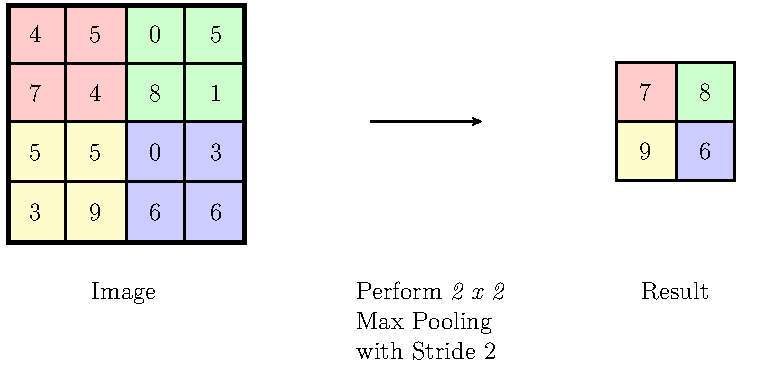
\includegraphics{images/pooling.pdf}
	\caption[Max pooling with $2 \times 2$ filter and stride $2$]{Max pooling with $2 \times 2$ filter $\vec{K}_{\text{max}}$ across a $4 \times 4$ input $\vec{I}$ with a stride of $s=2$. Within each window, the maximum of its values is computed. Finally, this yields a matrix with each maximum at its corresponding position.}
	\label{fig:pooling}
\end{figure}